\documentclass[12pt]{article}
\usepackage[utf8]{inputenc}
\usepackage{amsmath, amssymb, amsfonts}
\usepackage{graphicx}
\usepackage{listings}
\usepackage{xcolor}
\usepackage{geometry}
\usepackage{float}
\usepackage{subcaption}
\geometry{a4paper, margin=1in}

% تنظیمات ظاهر کدها در گزارش
\definecolor{codegray}{rgb}{0.5,0.5,0.5}
\lstset{
	language=Python,
	basicstyle=\ttfamily\small,
	commentstyle=\color{codegray},
	keywordstyle=\color{blue},
	numbers=left,
	frame=single,
	breaklines=true,
	postbreak=\mbox{\textcolor{red}{$\hookrightarrow$}\space}
}

\title{Project Report: Anime Recommendation System}
\author{Hediyeh Nayebi}

\renewcommand{\topfraction}{0.9}	% اجازه می‌دهد تا 90% بالای صفحه عکس باشد
\renewcommand{\bottomfraction}{0.8}	% اجازه می‌دهد تا 80% پایین صفحه عکس باشد
\renewcommand{\textfraction}{0.05}	% اجازه می‌دهد متن خیلی کم باشد

\begin{document}
	
	\maketitle
	
	\section{Introduction}
	
	In the contemporary digital era, the proliferation of online content has necessitated the development of sophisticated recommendation systems to assist users in navigating vast information spaces. Among these, the anime domain presents a unique challenge due to the diverse preferences of the user base and the hierarchical nature of anime metadata. 
	
	This project aims to design and implement a robust recommendation engine tailored for the anime dataset. The core objective is to move beyond simple popularity-based suggestions by leveraging Collaborative Filtering (CF) techniques. By analyzing user-item interaction patterns—specifically rating behaviors—we aim to uncover latent features that drive user preferences. 
	
	The primary contributions of this report are threefold:
	\begin{enumerate}
		\item \textbf{Data Exploration:} A comprehensive analysis of user-item interaction matrices to understand sparsity and interaction distributions.
		\item \textbf{Noise Reduction:} Implementation of data preprocessing techniques to mitigate the "cold-start" problem and improve dataset quality.
		\item \textbf{Model Evaluation:} Development and assessment of recommendation algorithms, evaluated against standard metrics such as Root Mean Square Error (RMSE) to ensure prediction accuracy.
	\end{enumerate}
	
	Through this systematic approach, we intend to provide a scalable and effective solution capable of delivering personalized recommendations within the high-dimensional anime ecosystem.
	\newpage
	\section{Data Exploration and Matrix Analysis}
	
	To understand the dataset structure, we performed an initial analysis of the user-item interaction matrix. The following Python code was used to calculate the matrix density and sparsity:
	
	\begin{lstlisting}[caption=Calculating Matrix Sparsity]
		# Calculate dimensions
		num_users = rating_df['user_id'].nunique()
		num_animes = rating_df['anime_id'].nunique()
		total_ratings = len(rating_df)
		
		# Sparsity calculation
		density = total_ratings / (num_users * num_animes)
		sparsity = 1 - density
		
		print(f"Matrix Sparsity: {sparsity * 100:.2f}%")
	\end{lstlisting}
	
	\subsection{Visualizing the Long Tail}
	We visualized the interaction frequency to identify the "Long Tail" phenomenon, where a small number of anime titles receive a disproportionate number of ratings.
	
	\begin{lstlisting}[caption=Plotting Interaction Frequency]
		# Plotting the Long Tail distribution
		anime_popularity = rating_df.groupby('anime_id')['rating'].count()
		plt.plot(np.sort(anime_popularity.values))
		plt.yscale('log') # Log scale to handle the skewness
		plt.title('Anime Interaction Frequency (Long Tail)')
		plt.show()
	\end{lstlisting}
	
\subsection{Mathematical Context}
The interaction dataset is modeled as a matrix $R \in \mathbb{R}^{U \times I}$, where $U$ denotes the set of users, $I$ denotes the set of anime titles, and $r_{ui}$ represents the rating given by user $u$ to anime $i$. 

Given that most users interact with only a tiny fraction of the available anime, $R$ is extremely sparse. The sparsity is mathematically defined as:
\begin{equation}
	\text{Sparsity} = 1 - \frac{|\{r_{ui} \mid r_{ui} \neq 0\}|}{|U| \times |I|}
\end{equation}

Furthermore, the interaction frequency visualized in the long-tail plot follows a power-law distribution. This is expressed as $P(x) \propto x^{-\alpha}$, indicating that a highly skewed minority of items receives the vast majority of interactions.
	
	\begin{figure}[H] % محیط اول برای نمودار اول
		\centering
		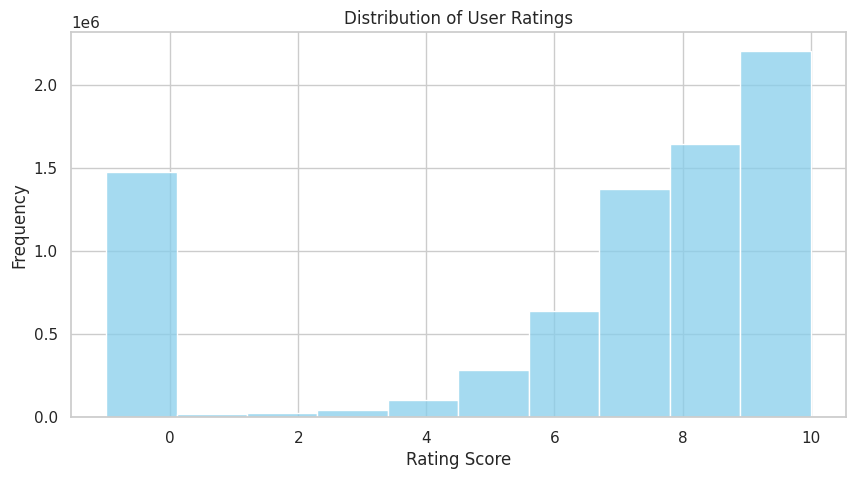
\includegraphics[width=0.8\textwidth]{../figures/my_image.png}
		\caption{Distribution of User Ratings}
	\end{figure}
	
	\begin{figure}[H] % محیط دوم برای نمودار دوم
		\centering
		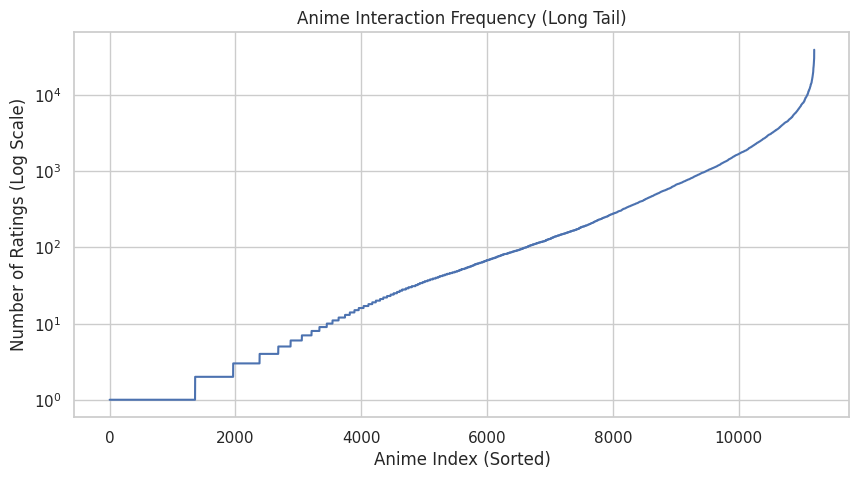
\includegraphics[width=0.8\textwidth]{../figures/my_image2.png}
		\caption{Long Tail Frequency (Logarithmic Scale)}
	\end{figure}
	
	\section{Data Preprocessing \& Noise Reduction}
	To address the cold-start problem and mitigate the computational challenges imposed by the high sparsity of the user-item interaction matrix, a robust data filtering pipeline was implemented. In collaborative filtering systems, users with very few interactions often introduce high noise and minimal signal, which severely limits the model's ability to learn stable and reliable preference profiles.
	
	Therefore, an activity threshold $\tau$ is defined such that any user $u$ with a total number of interactions less than $\tau$ is excluded from the active dataset. Formally, let $R_u = \{i \in I \mid r_{ui} \neq 0\}$ represent the set of items rated by user $u$. The filtering criterion for the active user base is expressed as:
	\begin{equation}
		U_{\text{filtered}} = \{u \in U \mid |R_u| \ge \tau\}
	\end{equation}
	
	For this implementation, the threshold was set to $\tau = 50$. This preprocessing step ensures that the recommendation engine trains exclusively on high-quality user profiles with well-established historical preferences, thereby significantly reducing matrix sparsity and optimizing computational efficiency.
	
\section{Data Preprocessing \& Noise Reduction}
To address the cold-start problem and mitigate the computational challenges imposed by the high sparsity of the user-item interaction matrix, a robust data filtering pipeline was implemented. In collaborative filtering systems, users with very few interactions often introduce high noise and minimal signal, which severely limits the model's ability to learn stable and reliable preference profiles.

Therefore, an activity threshold $\tau$ is defined such that any user $u$ with a total number of interactions less than $\tau$ is excluded from the active dataset. Formally, let $R_u = \{i \in I \mid r_{ui} \neq 0\}$ represent the set of items rated by user $u$. The filtering criterion for the active user base is expressed as:

$$ U_{\text{filtered}} = \{u \in U \mid |R_u| \ge \tau\} $$

For this implementation, the threshold was set to $\tau = 50$. This preprocessing step ensures that the recommendation engine trains exclusively on high-quality user profiles with well-established historical preferences, thereby significantly reducing matrix sparsity and optimizing computational efficiency.

The quantitative impact of this filtering process on the dataset dimensions is summarized in Table~\ref{tab:dataset_stats}.

\begin{table}[h!]
	\centering
	\caption{Dataset Statistics Before and After Noise Reduction ($\tau = 50$)}
	\label{tab:dataset_stats}
	\begin{tabular}{|l|r|r|r|}
		\hline
		\textbf{Metric} & \textbf{Original Dataset} & \textbf{Filtered Dataset} & \textbf{Impact (\% Change)} \\ \hline
		Total Ratings   & 7,813,737                 & 7,166,253                 & -8.29\%                     \\ \hline
		Unique Users    & 73,515                    & 39,466                    & -46.32\%                    \\ \hline
	\end{tabular}
\end{table}
	
\end{document}